\documentclass[tikz]{standalone}
\usepackage{tikz}
\usepackage{alphalph}
\usetikzlibrary{positioning, graphs}
\usetikzlibrary{graphs.standard}
\begin{document}
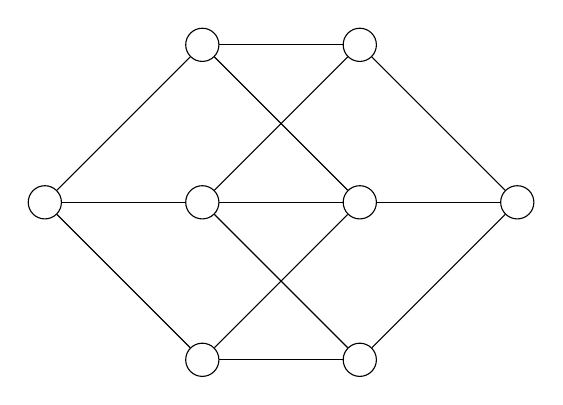
\begin{tikzpicture}
\begin{scope}
		[vertex/.style={draw,circle,inner sep = 0em, minimum size = 1.2em},
		 edgelabel/.style = {fill = white, inner sep = 0.2em, font=\small}]
		\node[vertex] (s) at (0, 0) {};
		\node[vertex] (a) at (2,  2) {};
		\node[vertex] (b) at (4,  2) {};
		\node[vertex] (c) at (2, 0) {};
		\node[vertex] (d) at (4, 0) {};
		\node[vertex] (e) at (2, -2) {};
		\node[vertex] (f) at (4, -2) {};
		\node[vertex] (t) at (6, 0) {};
		
        \draw[-] (s) to (a);
        \draw[-] (s) to (c);
        \draw[-] (s) to (e);
        \draw[-] (a) to (b);
        \draw[-] (a) to (d);
        \draw[-] (c) to (b);
        \draw[-] (c) to (d);
        \draw[-] (c) to (f);
        \draw[-] (e) to (d);
        \draw[-] (e) to (f);
        \draw[-] (b) to (t);
        \draw[-] (d) to (t);
        \draw[-] (f) to (t);
		
\end{scope}
\end{tikzpicture}
\end{document}